\documentclass{beamer}
\usepackage{listings}
\lstset{
%language=C,
frame=single, 
breaklines=true,
columns=fullflexible
}
\usetheme[progressbar=frametitle]{metropolis}
\usepackage{appendixnumberbeamer}

\usepackage{booktabs}
\usepackage[scale=2]{ccicons}
\newenvironment{subcolumns}[1]
 {\valign\bgroup\hsize=#1##\cr}
 {\crcr\egroup}
\newcommand{\nextsubcolumn} {\cr\noalign{\hfill}}
\newcommand{\nextsubfigure}{\vfill}
\usepackage{pgfplots}
\usepgfplotslibrary{dateplot}

\usepackage{xspace}
\newcommand{\themename}{\textbf{\textsc{metropolis}}\xspace}
\usepackage{subcaption}
\usepackage{url}

\usepackage{tikz}
\usetikzlibrary{arrows.meta,positioning}
\usepackage{pgfplots}
\pgfplotsset{compat=1.17}
\usepackage{tkz-fct}
\usepackage{mathrsfs}
\usepackage{txfonts}
\usepackage{tkz-euclide} 
\usetikzlibrary{calc,math}
\usepackage{float}
\newcommand\norm[1]{\left\lVert#1\right\rVert}
\renewcommand{\vec}[1]{\mathbf{#1}}
\providecommand{\pr}[1]{\ensuremath{\Pr\left(#1\right)}}
\usepackage[export]{adjustbox}
\usepackage[utf8]{inputenc}
\usepackage{amsmath}
\usepackage{mathtools}
\usepackage{xfrac}
\newcommand{\SubItem}[1]{
    {\setlength\itemindent{15pt} \item[-] #1}
}
\title{Real Data Analysis}
\subtitle{MA4740 - Introduction to Bayesian Statistics}
\date{\today}

\author{GROUP-2}
%\institute{Indian Institute of Technology Hyderabad}
\titlegraphic{\hfill
\includegraphics[height=1.5cm]{Images/iith logo.png}}

\begin{document}
\metroset{block=fill}
\begin{frame}
\titlepage
\end{frame}
\begin{frame}{Team Members}
\begin{itemize}
    \item Anita Dash - MA20BTECH11001
    \item Chilukuri Krishna Teja - MA20BTECH11005
    \item Kethari Narasimha Vardhan - MA20BTECH11006
\end{itemize}
\end{frame}
\begin{frame}
\section{Introduction}
\end{frame}
\begin{frame}{Introduction}
   \begin{block}{Abstract}
     This presentation is based on a group project part of the MA4740 - Introduction to Bayesian Statistics course material. The primary goal of this project is to acquire a real-world data set (not synthetic) and execute Beta Binomial Bayesian Analysis and other approaches presented in class.
   \end{block} 
\end{frame}
\begin{frame}{Introduction}
   \begin{block}{Objective}
    The project includes:
    \begin{itemize}
    \item Real Data Analysis on Dataset  MSFT stocks using method of moments and Maximum Likelihood approach
    \item Performing Beta-Binomial Bayesian Analysis on the Dataset MSFT stocks
\end{itemize}
   \end{block} 
\end{frame}
\begin{frame}
\section{Data Collection}
\end{frame}
\begin{frame}{Data Collection}
   \textbf{The Dataset}
     \begin{itemize}
    \item The Dataset, MSFT stocks which is based on the stocks of MSFT (Microsoft Corp)  has been taken from the Python3 \textit{yfinance} package.
    \item The data includes opening price, closing price, maximum price, minimum price and date. Amongst which, the attributes that are of our interest are closing price and date.
\end{itemize}
\begin{figure}[htp]
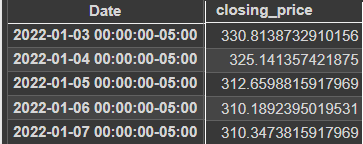
\includegraphics[width=0.475\textwidth]{Images/Glimpse.png}
\caption{Glimpse of the Dataset}
\end{figure}  
\end{frame}
\begin{frame}
\section{Beta-Binomial Bayesian Data Analysis}
\end{frame}
\begin{frame}{Prior-Data}
\begin{itemize}
    \item The prior data is on the stocks of MSFT from the year 2000 to 2022.
    \item The closing price of MSFT stocks on each day throughout the years is considered.
    \item Based on this prior data, we attempt to predict if MSFT's stock will rise or fall on a specific day after 2022.  
\end{itemize}
\end{frame}
\begin{frame}{Prior-Data}
\begin{itemize}
    \item The Prior Dataset is made up of the fraction of stock increases in each quarter from year 2000 to 2022.
    \item If the stock has increased from the previous day, the value is 1, otherwise it is 0.
    \item We choose a random variable $X$, where $X$ is the proportion of days the stock price increased in $n$ days, and $P(X = x)$ representing the probability of the proportion, $x$.  
\end{itemize}
\begin{block}{Example}
    Suppose in the past $n$ days, the MSFT stock has increased $k$ times, then
\begin{center}
    $x = \frac{k}{n}$
\end{center}
\end{block} 
\end{frame}
\begin{frame}{Prior-Data}
\begin{figure}[htp]
\centering
\begin{subcolumns}{0.475\columnwidth}
  \begin{subfigure}{0.46\columnwidth}
  \centering
  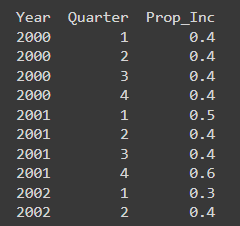
\includegraphics[width=\textwidth]{Images/Prior_Data.png}
  \caption{Glimpse of Prior Dataset}
  \end{subfigure}
\nextsubcolumn
  \begin{subfigure}{0.5\columnwidth}
  \centering
  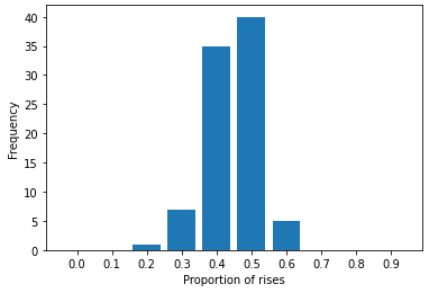
\includegraphics[width=\textwidth]{Images/FreqVsRise.png}
  \caption{prior data}
  \end{subfigure}
\end{subcolumns}
\end{figure}
We can see that the plot between the proportions with its frequency gives us a near normal distribution.
\end{frame}
\begin{frame}
\section{Data Analysis on Prior-Data using MOM and MLE}
\end{frame}
\begin{frame}{Method Of Moments (MOM)}
    \begin{block}{Formula}
    We can see that $X \sim N(\mu,\sigma)$ and $x_i$ are i.i.d realized values of $X$\\
    and hence we know that,
    \begin{center}
    $M1=E[X] = \mu = \frac{1}{n}\Sigma x_{i}$  
\end{center}

\begin{center}
    $M2=E[X^2] = \mu^2 + \sigma^2 = \frac{1}{n}\Sigma x_{i}^{2}$
\end{center}
    \end{block}
The calculations yield us the results
\begin{itemize}
    \item M1 = Mean ($\mu$) = 0.447727
    \item M2 = 0.206136
    \item Variance = 0.0057
    \item Standard Deviation$(\sigma)$ = 0.075344
\end{itemize}
\end{frame}
\begin{frame}{Maximum Likelihood Estimators (MLE)}
\begin{block}{definition}
Suppose $X \sim N(\mu,\sigma)$ and $x_i$ are i.i.d realized values of $X$\\
Then the likelihood function is,\\
\begin{center}
    $L(\theta|k) = \prod_{i=1}^n f(x_i|\theta_1,...,\theta_k)$
\end{center}
And the Maximum Likelihood Estimator(MLE) is,
\begin{center}
    $\hat{\theta}_{mle} = argmax_{\theta} L(\theta|x)$
\end{center}
    
\end{block}  
\end{frame}
\begin{frame}{Maximum Likelihood Estimators (MLE)}
\begin{block}{MLE of normal distribution}
The likelihood function,
\begin{center}
    $L(\theta, \sigma^2|X) = \prod_{i=1}^n f(x_i|\theta,\sigma^2)\\
    \implies L(\theta, \sigma^2|X) = \prod_{i=1}^n (\frac{1}{\sqrt(2\pi\sigma^2)}e^{\frac{-(x-\theta)^2}{2\sigma^2}})\\
    \log(L(\theta, \sigma^2|X)) = -\frac{n}{2}\log(2\pi)  -\frac{n}{2}\log(\sigma^2)  -\frac{1}{2\sigma^2}\sum_{i=1}^{n}(x_i-\theta)^2$
\end{center}
For a given $\sigma^2$, the log likelihood function is maximized when,
\begin{center}
 $\frac{\partial \log(L(\theta, \sigma^2|X))}{\partial \theta} = 0 \\
  \implies \sum_{i=1}^{n}(x_i-\theta) = 0
  \implies \theta = \frac{ \sum x_i}{n}$
\end{center}
Therefore, $\theta = \Bar{X}$
\end{block}
\end{frame}
\begin{frame}{Maximum Likelihood Estimators (MLE)}
\begin{block}{MLE of normal distribution}
For a given $\theta$, the log likelihood function is maximized when,
\begin{center}
 $\frac{\partial \log(L(\theta, \sigma^2|X))}{\partial \sigma^2} = 0 \\
  \implies -\frac{n}{2\sigma^2} + \frac{1}{2(\sigma^2)^2}(\sum_{i=1}^{n}(x_i-\theta)^2) = 0\\
  \implies \sigma^2 = \frac{1}{n}\sum_{i=1}^{n}(x_i-\theta)^2 \\
  \implies  \sigma^2 = \frac{1}{n}\sum_{i=1}^{n}(x_i^2) - \theta^2$
\end{center}
Therefore, $\sigma^2 = \frac{1}{n}\sum_{i=1}^{n}(x_i^2) - \theta^2$
\end{block}
\end{frame}
\begin{frame}{Maximum Likelihood Estimators (MLE)}
\begin{center}
    Our distribution is a normal distribution, and we have shown that the MOM and MLE yield the same result.
\end{center}
\begin{figure}[htp]
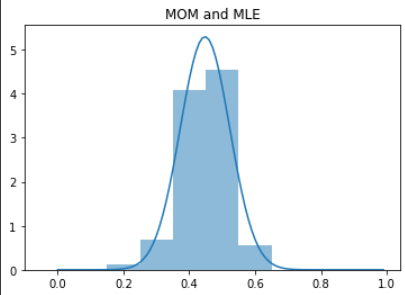
\includegraphics[width=0.65\textwidth]{Images/MOM_MLE.png}
\caption{MOM and MLE}
\end{figure}  
\end{frame}
\begin{frame}
\section{Beta Distribution}
\end{frame}

\begin{frame}{Beta Distribution}
We try to fit our prior-data distribution to a beta distribution.\\
We get $X \sim Beta(\alpha, \beta)$, where,
\begin{block}{Formula}
    \begin{center}
    mean$(\mu) = \frac{\alpha}{\alpha + \beta}$ \\
    var$(\sigma) = \frac{\alpha\beta}{(\alpha + \beta)^2(\alpha + \beta + 1)}$
\end{center}
\end{block}
\end{frame}

\begin{frame}{Beta Distribution}
Using the values of $\mu$ and $\sigma$ found earlier using MOM and MLE. We get the following values of $\alpha$ and $\beta$
\begin{center}
    $\alpha = 19.055$,   
    $\beta = 23.504$\\
    prior mean $= 0.4477$
\end{center}  
\begin{figure}[htp]
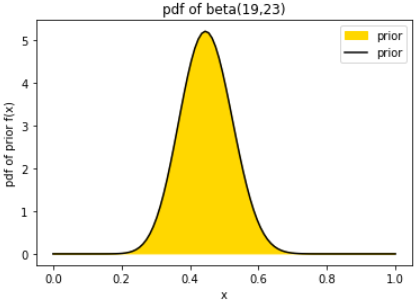
\includegraphics[width=0.55\textwidth]{Images/Pdf_beta_prior.png}
\caption{PDF of $\beta(19,23)$}
\end{figure}
\end{frame}
\begin{frame}
\section{Data-Likelihood Function}
\end{frame}
\begin{frame}{Data-Likelihood Function}
\begin{itemize}
    \item We require a likelihood function to perform a beta-binomial analysis on the generated beta distribution. 
    \item We choose $L \mid \pi \sim Bin(n,\pi)$ where,
    \begin{center}
    \begin{small}
    $n$: The number of days we are looking at to see if the stock price has increased or decreased \\
    $\pi$: the Probability that the stock price will increase
    \end{small}
    \end{center}
    \item Our data consists of the realized proportion of increase in stocks in the year 2022, where
    \begin{center}
    \begin{small}
    $n$ = 251 \\
    $y$ = 116\\
    $p$ = 0.46215
    \end{small}
    \end{center}
\end{itemize}
\end{frame}
\begin{frame}{Plot of Distributions}
\begin{figure}[htp]
\centering
\begin{subcolumns}{0.47\columnwidth}
  \begin{subfigure}{0.47\columnwidth}
  \centering
  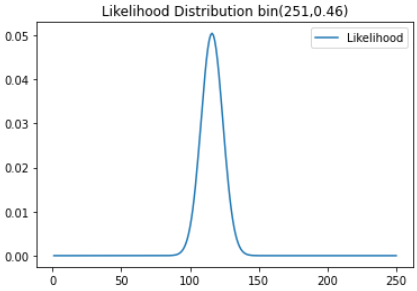
\includegraphics[width=\textwidth]{Images/Likelihood_Dist.png}
  \caption{Plot of Likelihood Function}
  \end{subfigure}
\nextsubcolumn
  \begin{subfigure}{0.5\columnwidth}
  \centering
  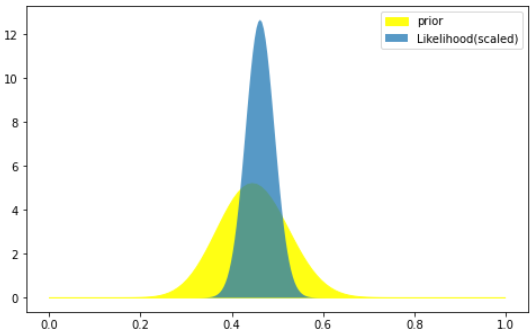
\includegraphics[width=\textwidth]{Images/Prior_Likelihood.png}
  \caption{Plot of Prior Distribution and Likelihood Function (Scaled)}
  \end{subfigure}
\end{subcolumns}
\end{figure}  
\end{frame}
\begin{frame}
\section{Posterior Distribution}
\end{frame}
\begin{frame}{Posterior Distribution}
   We Find the posterior distribution using the prior data and the likelihood function. 
   \begin{block}{Definition}
       If the,
       \begin{center}
         Prior: $\pi \sim Beta(\alpha,\beta)$\\
       Data-Likelihood: $Y|\pi \sim Bin(n,\pi)$\\
       \end{center}
       Then the,
       \begin{center}
       Posterior: $\pi|(Y=y) \sim Beta(\alpha + y,\beta + n - y)$  
       \end{center} 
   \end{block}
Where, $y$ is the realized value of number of times stocks increased in $n$ days
\end{frame}
\begin{frame}{Posterior Distribution}
Thus, after performing the necessary calculations, we get 
\begin{center}
\begin{small}
posterior alpha = 135.055\\
posterior beta = 158.504\\
Posterior mean = 0.46006     
\end{small}
\end{center}
\begin{figure}[htp]
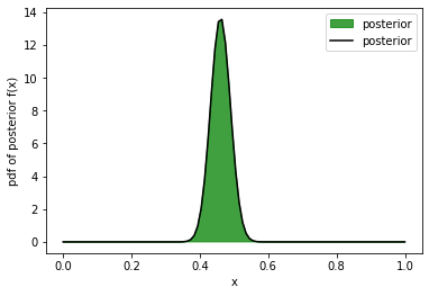
\includegraphics[width=0.6\textwidth]{Images/Posterior_Dist.png}
\caption{PDF of posterior distribution}
\end{figure}
\end{frame}
\begin{frame}{Conclusion}
From the below combined plot we can see that the mean of our prior and posterior differ by 0.02 which is not that high. But the variance of prior and posterior differ by a lot.

        \begin{align*}
        \textit{Prior std} = 0.07534356570114019\\
        \textit{Post std} = 0.029039831153004316
        \end{align*}

        \begin{align*}
        \textit{Prior estimation of proportion} \approx \left (29.704\%, 59.841\% \right )\\
        \textit{Posterir estimation of proportion} \approx \left (40.198\%, 51.813\% \right )
        \end{align*}
\end{frame}
\begin{frame}{Conclusion}
\begin{figure}[htp]
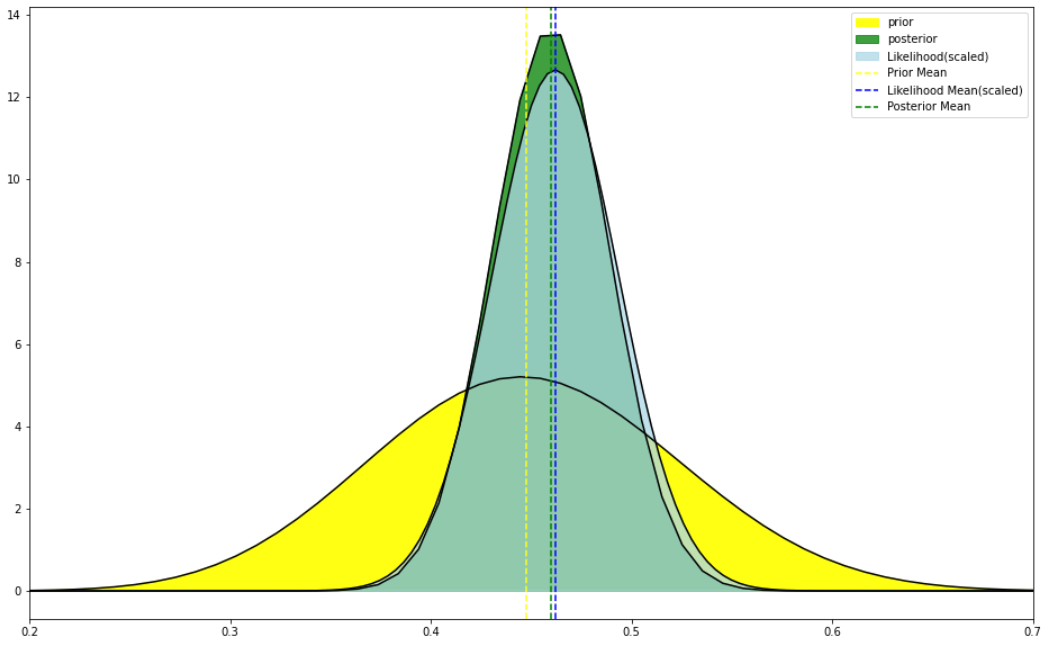
\includegraphics[width=\textwidth]{Images/Final_Comb_Plot.png}
\caption{}
\end{figure}  
\end{frame}
\begin{frame}
\section{Thank You}  
    \begin{center}     \href{https://colab.research.google.com/drive/1AMuKl883Mes_bpji0VLkH9uxfi8i9bwj?usp=sharing}{\beamergotobutton{Source Code}}
    \end{center}
\end{frame}
\end{document}
